%% hugo-title: Predoc Placement (LaTeX)
%% hugo-date: 2026-07-15
%% hugo-draft: false

\documentclass[11pt]{article}
%% Shared Tufte-inspired preamble — matches site colorway
\usepackage[T1]{fontenc}
\usepackage{lmodern}
\usepackage{amsmath,amssymb}
\usepackage{graphicx}
\usepackage{booktabs}
\usepackage{microtype}
\usepackage[
  paperwidth=6.5in,
  top=1.4in,
  bottom=1.4in,
  left=1in,
  right=2.75in,
  marginparwidth=1.75in,
  marginparsep=0.2in
]{geometry}

\usepackage{xcolor}
\definecolor{textcolor}{RGB}{39,39,39}
\definecolor{linkcolor}{RGB}{26,13,171}
\definecolor{rulecolor}{RGB}{39,39,39}

\usepackage[colorlinks=true,linkcolor=linkcolor,citecolor=linkcolor,urlcolor=linkcolor]{hyperref}

\usepackage{tikz}
\usetikzlibrary{arrows.meta,calc}

\pagestyle{empty}
\setlength{\parindent}{0pt}
\setlength{\parskip}{0.65\baselineskip}
\color{textcolor}

%% Section spacing (Tufte-inspired, no extra packages)
\makeatletter
\renewcommand\section{\@startsection{section}{1}{0pt}{1.25\baselineskip}{0.5\baselineskip}{\large\bfseries\color{textcolor}}}
\renewcommand\subsection{\@startsection{subsection}{2}{0pt}{1\baselineskip}{0.35\baselineskip}{\normalsize\bfseries\color{textcolor}}}
\makeatother

%% Margin notes (Tufte sidenotes)
\newcommand{\sidenote}[1]{\marginpar{\footnotesize\color{textcolor}#1}}

%% TL;DR block
\newcommand{\tldr}[1]{%
  \noindent{\color{linkcolor}\textit{TL;DR}}\textit{ #1}\par\vspace{0.5\baselineskip}%
}

%% Figure styling
\usepackage{caption}
\captionsetup{
  font=small,
  labelfont=bf,
  textfont=it,
  skip=0.5\baselineskip
}


\begin{document}

\tldr{A practice conversion of the predoc-placement post into \LaTeX{}. System to analyze CVs from 15 top economics PhD programs: about two-thirds of students had predoc experience, and the Fed, NBER, and top business schools are the most common predoc institutions.}

\section{Key findings}

A CV-analysis pipeline covering 100 students across 15 economics PhD programs (2018--2024) shows predoc experience is now the norm rather than the exception.

\begin{table}[ht]
\centering
\begin{tabular}{@{}lr@{}}
\toprule
Metric & Value \\
\midrule
Total students analyzed & 100 \\
Universities covered & 15 \\
Students with predoc experience & 67\% \\
Year range & 2018--2024 \\
\bottomrule
\end{tabular}
\caption{Summary statistics.}
\end{table}

\section{Top predoc institutions}

The Federal Reserve Board and NBER are the most common predoc placements, followed closely by top business-school research programs.

\begin{figure}[ht]
\centering
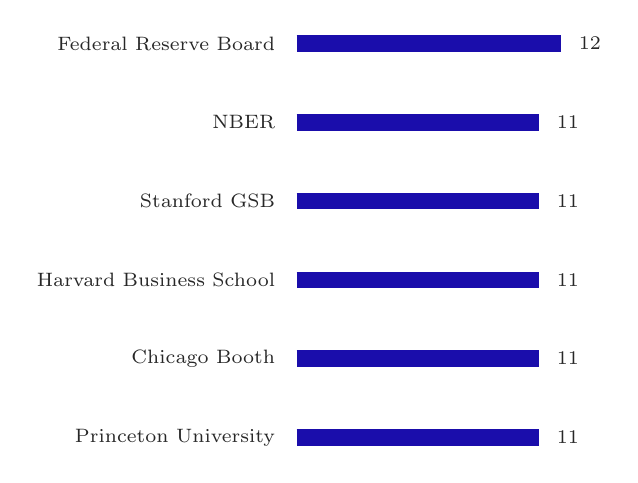
\begin{tikzpicture}[scale=1, every node/.style={color=textcolor, font=\footnotesize}]
  \draw[linkcolor, line width=6pt] (0,5.5) -- (3.36,5.5);
  \node[anchor=east, font=\scriptsize] at (-0.15,5.5) {Federal Reserve Board};
  \node[anchor=west, font=\scriptsize] at (3.46,5.5) {12};

  \draw[linkcolor, line width=6pt] (0,4.5) -- (3.08,4.5);
  \node[anchor=east, font=\scriptsize] at (-0.15,4.5) {NBER};
  \node[anchor=west, font=\scriptsize] at (3.18,4.5) {11};

  \draw[linkcolor, line width=6pt] (0,3.5) -- (3.08,3.5);
  \node[anchor=east, font=\scriptsize] at (-0.15,3.5) {Stanford GSB};
  \node[anchor=west, font=\scriptsize] at (3.18,3.5) {11};

  \draw[linkcolor, line width=6pt] (0,2.5) -- (3.08,2.5);
  \node[anchor=east, font=\scriptsize] at (-0.15,2.5) {Harvard Business School};
  \node[anchor=west, font=\scriptsize] at (3.18,2.5) {11};

  \draw[linkcolor, line width=6pt] (0,1.5) -- (3.08,1.5);
  \node[anchor=east, font=\scriptsize] at (-0.15,1.5) {Chicago Booth};
  \node[anchor=west, font=\scriptsize] at (3.18,1.5) {11};

  \draw[linkcolor, line width=6pt] (0,0.5) -- (3.08,0.5);
  \node[anchor=east, font=\scriptsize] at (-0.15,0.5) {Princeton University};
  \node[anchor=west, font=\scriptsize] at (3.18,0.5) {11};
\end{tikzpicture}
\caption{Number of admitted students who completed a predoc at each institution.}
\end{figure}

\sidenote{Counts are admitted students who completed a predoc at that institution before starting their PhD, not total predoc positions offered.}

\section{Code}

\href{https://github.com/mwballif/phd-cv-analyzer}{github.com/mwballif/phd-cv-analyzer} --- scrapers, database, Streamlit dashboard, export/analysis tools.

\end{document}
